\documentclass{article}

\usepackage{amsmath}
\usepackage{gensymb}
\usepackage{graphicx}
\usepackage{caption}

\title{Programming and Data Analysis Assignment 2: The Hubble Constant}
\author{Elliott Ashby}
\date{\today}


\begin{document}
    \maketitle

    \section{Step 1}
    In order to obtain the Cepheid period-luminosity (PL) relation, two constants, $\alpha$ and $\beta$ needs to be determined
    to form the equation;
    \begin{equation}
        M = \alpha \log P + \beta
    \end{equation}
    Where $M$ is absolute magnitude and $P$ is period. \newline
    Therefore, in order to find these two constants, a fit must be determined relating $M$ and $\log P$ in the form of $y = mx + c$. \newline
    \newline
    Finding $\log P$ is trivial, simply take logarithms (in this case of base 10) of all values of $P$. \newline
    Finding $M$ is slightly more in depth however. In order to convert our measured values of $m_{Apparent}$ to $M_{Absolute}$. \newline
    To convert between absolute and apparent magnitudes we can use;
    \begin{equation}
        M = m - 5 \log d_{pc} + 5 - A
    \end{equation}
    Where $d_{pc}$ distance from Earth in parsecs and $A$ is extinction. \newline
    While we have data for extinction values $A$, we don't have any values for distance from Earth $d_{pc}$. 
    These can be derived using parallax of the measured stars;
    \begin{equation}
        d_{pc} = 1000 / p_{mas}
    \end{equation}
    Where $p_{mas}$ is parallax of a star measured in milli-arcseconds. \newline
    \newline
    \begin{figure}
        \centering
        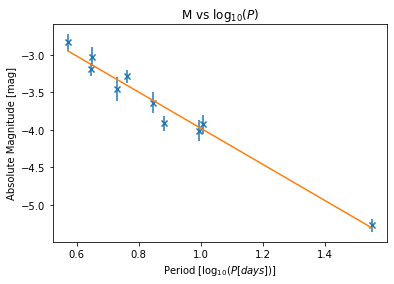
\includegraphics[scale = 0.7]{../media/images/part1.png}
        \caption{The relationship between Absolute Magnitude $M$ and logarithmic Period $\log P$}
    \end{figure}
    \textbf{Fig 1} shows relationship (1) along with propagated errors and a best fit. The fit has gradient
    $\alpha = -2.419 \pm 0.112$ and intercept $\beta = -1.550 \pm 0.104$ \newpage
    Performing a $\chi^2$ fit test on the data returns 10.66, with a $\chi^2_{red}$ of  1.18 which is acceptable 
    as a good fit as it lies in $1\pm\sqrt{\frac{2}{9}}$ This suggests that the $\alpha$ and $\beta$ values obtained are valid for this data set.
    \section{Step 2}
    To calculate the distance of the nearby galaxy NGC4527 we can use our new equation with constants;
    \begin{equation}
        M = -2.419 \pm 0.112 \log P -1.550 \pm 0.104
    \end{equation}
    along with (2) to find values of $d_{pc}$ for all data on NGC4527. \newline
    In order to gain a more precise approximation of NGC4527's distance from Earth, the data for body C1-V11 was removed as a statistical outlier since it was more than two times the standard deviation away from the average. \newline
    Since $\log P$ is already known, corresponding values of $M$ can be calculated. With these values and rearraging (2) to find $d_{pc}$ with $A = 0.0682$ (The extinction of NGC4527),
    values for $d_{pc}$ can be found for each data point in the galaxy of NGC4527. \newline
    \newline
    Calculating an average from both the values and the errors on each value returns a distance from Earth to NGC4527
    of $13.76 \pm 1.01 Mpc$. \newline
    This value however, is calculated from only one extinction value, in reality, each data point should have its own distinct extinction. This may skew the results in either positve or negative direction.

    \section{Step 3}
    In order to estimate the Hubble Constant and therefore the Expansion Rate of the Universe, we can use the simple relationship of Hubble's Law;
    \begin{equation}
        v_{rec} = H_0D_{gal}
    \end{equation}
    Where $v_{rec}$ is the recession velocity of a given galaxy, $H_0$ is the Hubble Constant and $D_{gal}$ is the distance from a given galaxy. \newline
    \newline In the case of NGC4527, $v_{rec} = 1152 kms^{-1}$. Given this, and using $d_{pc}$ of NGC4527 from step 2 as $D_{gal}$, the Hubble Constant can be estimated to be \newline $83.72 \pm 12.33 kms^{-1}Mpc^{-1}$
    \newline
    \newline This, of course, is a wildly inaccurate estimation due to the errors involved in it's calculation. To reduce these errors we can use more data to get a more acceptable Hubble Constant with a reduced error.
    \begin{figure}
        \centering
        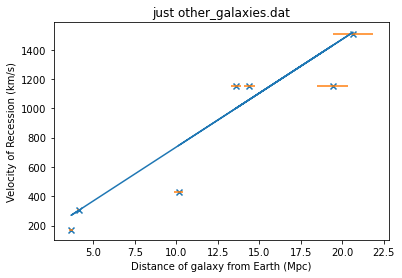
\includegraphics[scale = 0.7]{../media/images/part3.png}
        \caption{Recession Velocity ($v_{rec}$ in $km/s$) against galaxy's distance from Earth ($D_{gal}$ in $Mpc$) only including other\_galaxies.dat}
    \end{figure}
    \newline
    \newline
    Finding a fit of $y = mx$, with $y$ as $v_{rec}$, $m$ as $H_0$ and $x$ as $D_{gal}$ returns $H_0$ as $73.63 \pm 0.0001518 kms^{-1}Mpc^{-1}$ (see $\textbf{Figure 2}$)
    \newline
    \newline
    Additionally, if we combine this data with our data on NGC4527 from step 2 we can gain greater accuracy. Performing the same fitting on the new data set (see $\textbf{Figure 3}$)
    shows a slightly shallower gradient and $H_0$ of $71.07 \pm 0.0257 kms^{-1}Mpc^{-1}$.
    \begin{figure}
        \centering
        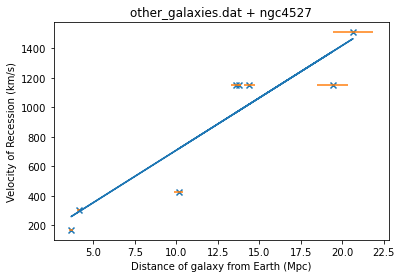
\includegraphics[scale = 0.7]{../media/images/part3.1.png}
        \caption{Recession Velocity ($v_{rec}$ in $km/s$) against galaxy's distance from Earth ($D_{gal}$ in $Mpc$) from other\_galaxies.dat and data from NGC4527}
    \end{figure}
    \newline 
    \newline 
    Performing a $\chi^2$ fit test on $\textbf{Figure 3}$ data produces a $\chi^2$ value of 429.3 with a $\chi^2_{red}$ of 61.33
    While this seems large, it should be accepted since the data clearly shows the trend of a positive correlation. We can add an intrinsic dispersion to the error of the calculated velocities equal to 147.
    This reduces $\chi^2$ to 7.029 and $\chi^2_{red}$ to 1.004. As this is within the range of $1\pm\sqrt{\frac{2}{7}}$ we can accept this model.
\end{document}